\item[(b)]
\section*{Task (b)}

\subsection*{Problem Statement}
Compute the spectrum for the whole signal length using the MATLAB command `fft`. Plot the magnitude of the spectrum. Label the axes correctly, with the frequency axis scale in Hz (Hint: the frequency values given in Table 1 should be visible at the correct position on the frequency axis).

\subsection*{Python Script}
\begin{verbatim}
import numpy as np
import matplotlib.pyplot as plt
from scipy.io import wavfile
import os

# Create fig directory if it doesn't exist
if not os.path.exists('fig'):
    os.makedirs('fig')

# Read the DTMF signal from the WAV file
fs, signal = wavfile.read('dtmf.wav')

# Compute the FFT for the whole signal length
spectrum = np.fft.fft(signal)
frequencies = np.fft.fftfreq(len(signal), 1/fs)

# Plot the magnitude spectrum
plt.figure(figsize=(10, 6))
plt.plot(frequencies[:len(frequencies) // 2], np.abs(spectrum[:len(frequencies) // 2]))
plt.title('Magnitude Spectrum of the Entire DTMF Signal')
plt.xlabel('Frequency (Hz)')
plt.ylabel('Magnitude')
plt.grid(True)
plt.savefig('fig/ex4_b_dtmf_spectrum.png')
plt.show()
\end{verbatim}

\subsection*{Magnitude Spectrum of the Entire DTMF Signal}
\begin{figure}[h]
    \centering
    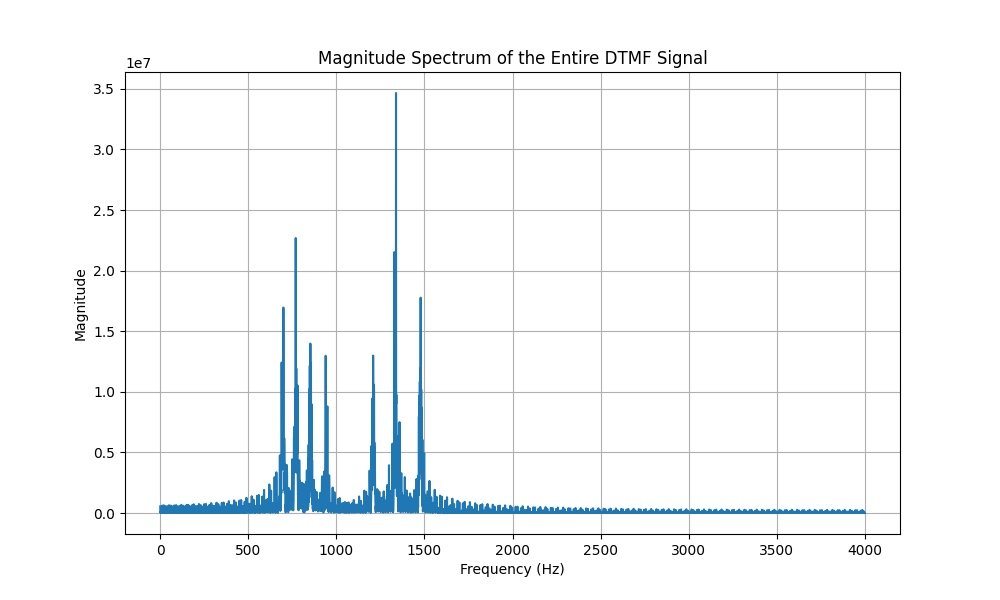
\includegraphics[width=0.8\textwidth]{fig/ex4_b_dtmf_spectrum.png}
    \caption{Magnitude Spectrum of the Entire DTMF Signal}
    \label{fig:ex4_b_dtmf_spectrum}
\end{figure}

\subsection*{Analysis}
The magnitude spectrum of the entire DTMF signal shows the frequencies present in the signal. The frequencies corresponding to the DTMF tones listed in Table 1 should be visible at the correct positions on the frequency axis, confirming the presence of these tones in the signal.
